% !TeX spellcheck = de_DE
\documentclass[ngerman,12pt]{article}

% Packages for Language
\usepackage[ngerman]{babel}
\usepackage[utf8]{inputenc}
\usepackage[T1]{fontenc}
\usepackage[final]{graphicx}
\usepackage{amsmath}
\usepackage{float}
%\usepackage{wrapfig}
\usepackage{caption}
%\usepackage{multirow}
\usepackage{subfig}
\usepackage{hyperref}
\usepackage[german, plain]{fancyref}
\usepackage{afterpage,pdflscape} %%% !!!!!!! CHANGE TO PDFLSCAPE LATER!
\usepackage{varioref}
\usepackage{siunitx}
\usepackage{translator}
\usepackage{listings}
\usepackage{fancyhdr}
\pagestyle{fancy}

%\usepackage{showframe}

\setlength{\headheight}{15.5pt}
\lhead{NAME NAME NAME}
\rhead{\today}
\chead{Numerik Übung 7}


\begin{document}
\lstset{language=Matlab,basicstyle=\ttfamily,columns=fixed}
\subsubsection*{adaptDivDiff.m}
\begin{lstlisting}[frame=single]
function [x, N] = adaptDivDiff(f, a, b, n)
  xp = linspace(a, b, 4097);
  x = [a; b];
  N = divDiff(x, f(x));
  xi = [0.5*(a+b)];
  fxi = f(xi);
  pxi = hornerNewton(N, x, xi);
  subplot(2, 1, 1)
  plot(xp, f(xp), 'r-', x, f(x), 'ks', ...
    xp, hornerNewton(N, x, xp), 'b--');
  title('Funktionen')
  subplot(2, 1, 2)
  plot(xp,abs(f(xp)-hornerNewton(N, x, xp)),'r-');
  title('Error')
  pause(1);
  for ii=2:n
    [~, jj] = max(abs(fxi-pxi));
    h = (xi(jj) - x(jj))/2;
    [x, N] = addDivDiff(x,N,xi(jj),fxi(jj));
    xi = [xi(jj)+h; xi(1:jj-1);...
          xi(jj)-h; xi(jj+1:end)];
    fxi = [f(xi(1)); fxi(1:jj-1);...
           f(xi(jj+1)); fxi(jj+1:end)];
    pxi = hornerNewton(N, x, xi);
    
    subplot(2, 1, 1)
    plot(xp, f(xp), 'r-', x, f(x), 'ks',...
         xp, hornerNewton(N, x, xp), 'b--');
    title('Funktionen')
    subplot(2, 1, 2)
    plot(xp,abs(f(xp)-hornerNewton(N,x,xp)),'r-');
    title('Error')
    pause(0.1);
  end
end
\end{lstlisting}

\subsubsection*{divDiff.m}
\begin{lstlisting}[frame=single]
function [ N ] = divDiff( x, y )
n=length(y);
N=y;
for i=1:n-1
  N(i+1:n)=(N(i+1:n)-N(i:n-1))./(x(i+1:n)-x(1:n-i));
end
end
\end{lstlisting}
%\filbreak
\subsubsection*{hornerNewton.m}
\begin{lstlisting}[frame=single]
function [ p ] = hornerNewton( N, x, xi )
n=length(N);
p=N(n)*ones(size(xi));
for i=n-1:-1:1
  p = p.*(xi-x(i))+N(i);
end
end
\end{lstlisting}

\subsubsection*{addDivDiff.m}
\begin{lstlisting}[frame=single]
function [xe, Ne] = addDivDiff(x, N, xi, yi)
xe = [xi; x];
Ne = zeros(size(N));
Ne(1)=yi;
for i=1:length(N)
  Ne(i+1) = (N(i)-Ne(i))/(x(i)-xi);
end
end
\end{lstlisting}

\subsubsection*{Output}
\begin{figure}[H]
    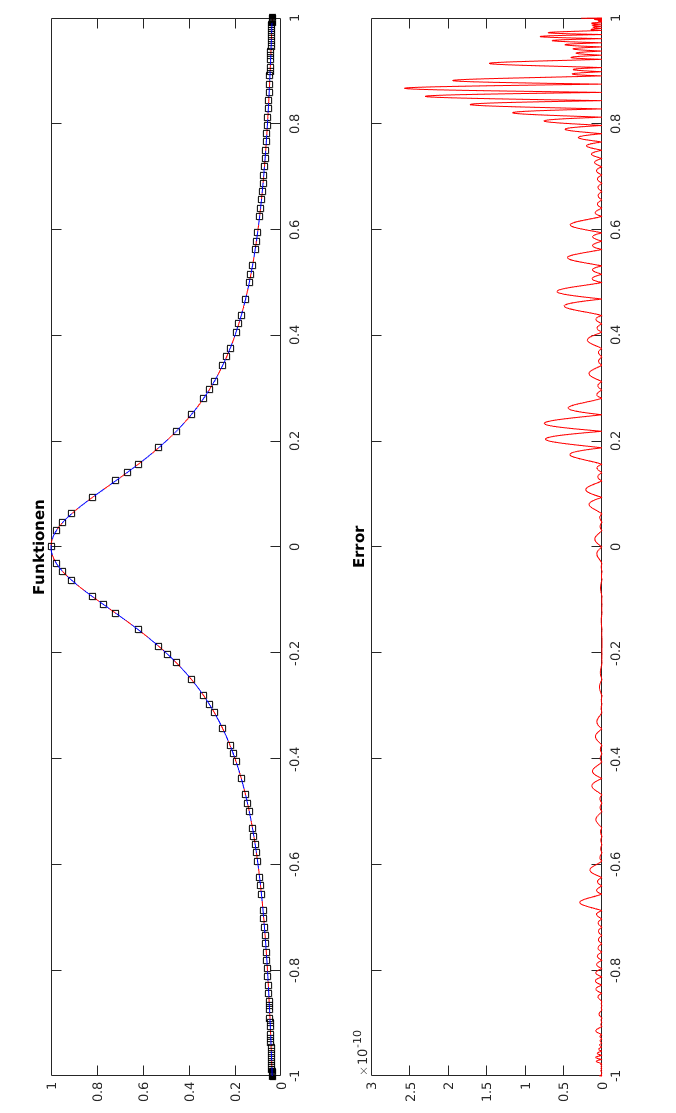
\includegraphics[height=0.93\textheight,keepaspectratio]{final_wf.png}
\end{figure}

\end{document}